For any kind of structure data, Strucured Query Language (SQL) is normally the best way of representing it, and we can immediatly understand that there are five core entities in our system:

\begin{enumerate}
  \item Tool - which represents the underlying tool used in the decomposition.
  \item Language - which represents which languages can be targeted for decomposition.
  \item Result - which represents if a given job of decomposition was successful or not.
  \item Decomposition - which represents the decomposition itself and all data required to represent it.
  \item Service - which represents each microservice.
\end{enumerate}

The relationships between them is represented in \Cref{fig:database-model}.

\begin{figure*}[!htb]
  \caption{Database Model}
  \label{fig:database-model}
  \centering
  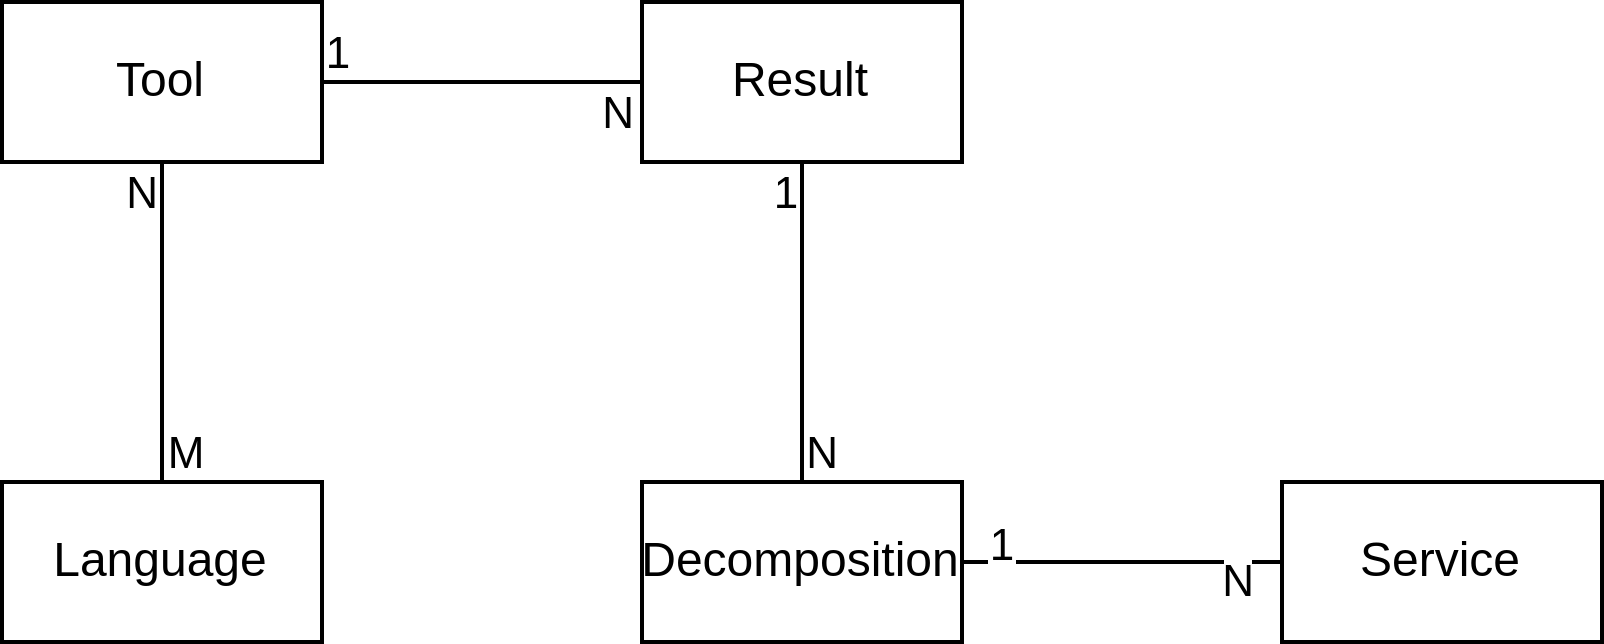
\includegraphics[width=\textwidth]{thesis-er.drawio}
\end{figure*}

